\section{Methodology of Random Forest}

The sentiment analysis base on RF pipeline can be visually and logically described with the following flowchart:

\begin{figure}[ht]
    \centering
    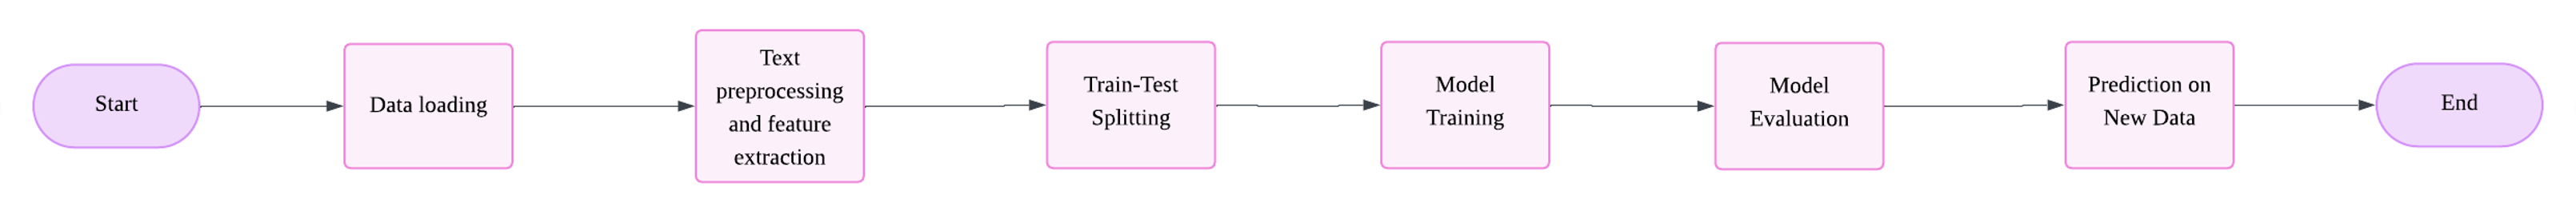
\includegraphics[width=1\textwidth]{pics/rf_steps.png}
    \caption{Random Forest analysis pipeline}
\end{figure}

\subsection{Step-by-step inputs and outputs}

\subsubsection{Dataset Loading}
The first step is acquiring the dataset. We use the IMDb movie review dataset which is available on HuggingFace under the ID "stanfordnlp/imdb". The data is loaded using the "load\_dataset" function from HuggingFace's datasets library. After loading, it is converted into a pandas DataFrame to facilitate further processing.

Input: Dataset is fetched automatically.\\
Process: Dataset is downloaded and parsed.\\
Output: A structured dataset with two columns: text (the review) and label (the sentiment class).

\subsubsection{Text Preprocessing and Feature Extraction}
Machine learning models cannot interpret raw textual data directly. Therefore, we must convert each review into a numerical representation. This is done using TF-IDF (Term Frequency-Inverse Document Frequency) vectorization.

TF-IDF calculates the importance of a word in a document relative to all other documents. We use the TF-IDF Vectorizer from scikit-learn configured with "max\_features" as 10000 to limit vocabulary size and stop\_words as 'english' to remove commonly used words that carry little sentiment meaning.
This process transforms the review texts into a high-dimensional sparse matrix, in this format, reviews are represented rows, the columns in every row are the features of words.

Input: Raw review texts and labels.\\
Process: Tokenization, stopword removal and TF-IDF computation.\\
Output: A TF-IDF feature matrix X\_vec with shape.

\subsubsection{Train-Test Splitting}
In this step, we split the dataset into two group for training and testing by "train\_test\_split" method of "scikit-learn" package. We allocate 80\% of the data to training and 20\% to testing. The split is randomized but reproducible due to a fixed random seed by setting "random\_state" as 42.
This step ensures that the model is trained on one collection of samples, and evaluated on another samples completely, which simulates a real-world scenario.

Input: TF-IDF feature matrix X\_vec and label vector y. \\
Process: Random partitioning of data into training and test sets. \\
Output: The group "X\_train" and "y\_train" for training, while the group "X\_test" and "y\_test" for evaluating.

\subsubsection{Model Training}
We train a classifier based on Random Forest, which is an ensemble algorithm. It generates several decision trees to predict together for more accurate results, this combination can also reduce overfitting. The classifier is instantiated using "RandomForestClassifier" of "scikit-learn" package. For the initial experiment, we use default settings with "n\_estimators" as 100, which means 100 decision trees are built. The training data, stored in the variables named as "X\_train" and "y\_train", is passing into the "fit" function, which constructs the trees by learning patterns in the TF-IDF features that differentiate positive and negative reviews.

Input: X\_train (TF-IDF vectors) and y\_train (labels). \\
Process: Each tree learns decision rules from data subsets and the forest aggregates these decisions.\\
Output: A trained RandomForestClassifier model object.

\subsubsection{Model Evaluation}
After training, the model with prediction ability is used to classify the samples we never seen before. This is done using the test set "X\_test" and "y\_test". We use the "predict" method to generate predicted labels and then calculate performance metrics. These metrics help understand both overall accuracy and error distribution which is especially important in binary classification tasks.

\begin{itemize}
    \item Accuracy: the proportion of correct predictions
    \item Classification Report: includes precision, recall and F1-score
    \item Confusion Matrix: shows the number of positives and negatives predictions with true or false
\end{itemize}

Input: Trained model, X\_test and y\_test. \\
Process: Predict labels and compare against true values \\
Output: Accuracy score, detailed classification report and confusion matrix.

\subsubsection{Prediction on New Data}
Finally, the model trained before is used to predict sentiment on other movie reviews provided by users. Before prediction, the new review text must go through the same TF-IDF transformation as the training data. The "vectorizer.transform" method is used to convert raw text to a vector which is then passed to the model's "predict" method.

Input: New review text. \\
Process: Apply TF-IDF vectorization, ten make prediction. \\
Output: A sentiment prediction 0 (negative) or 1 (positive).


\subsection{Implementation of Random forest}
The implementation of this sentiment analysis project is fully contained, which consists of the following key components.

\begin{enumerate}
    \item Loading the IMDb Dataset from HuggingFace: The script uses the datasets library to automatically fetch the standfordnlp/IMDb dataset. Only the labeled train and test splits are used. The data is then converted into pandas DataFrames for ease of manipulation and preprocessing.
    \item TF-IDF Vectorization: The textual content is convert into numerical features by using TF-IDF Vectorizer from scikit-learn. The vectorizer is configured with max\_features as 10000 and stop\_words as 'english' to ensure a compact, meaningful vocabulary. This transforms raw text into a sparse matrix of features suitable for machine learning.
    \item Model Training and Prediction Using Random Forest: A RandomForestClassifier is initialized with 100 decision trees. The training data set is used to fit this classifying model, then, the model is used to obtain predictions by testing data set.
    \item Evaluation Metrics Output: After prediction, the script computes accuracy score, confusion matrix, classification report including precision, recall and F1-score. These metrics provide a comprehensive insights about the performance of the model on unused data.
    \item Confusion Matrix Visualization and Saving: The confusion matrix is plotted as a heatmap for better readability and visual analysis. The resulting plot is saved as an image file.
\end{enumerate}


\subsection{Results of random forest}
In this section, we demonstrate the experimental data, which is gained from training and evaluating the Random Forest classifier on the IMDb movie review dataset. These experimental results are discussed in standard metrics such as accuracy, precision, recall, F1-score and confusion matrix.

After training, the model is evaluated on the preprocessed TF-IDF features of the unseen dataset. We gained the accuracy as 85.3\%, which shows that the Random Forest model is able to classify the sentiment of about 8.5 out of every 10 reviews correctly. Given the simplicity of the feature representation, this is a strong baseline.

\subsubsection{Classification Report}
\begin{figure}[ht]
    \centering
    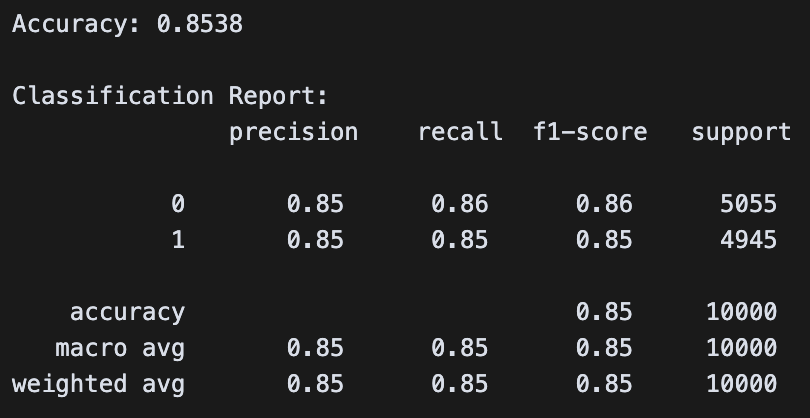
\includegraphics[width=0.5\textwidth]{pics/rf_eval_report_with_acc.png}
    \caption{Classification Report of Random Forest}
\end{figure}

Precision: When the model predicts a sentiment, it is correct about 85\% of the time. \\
Recall: The model is slightly lower at identifying positive reviews than negative ones. \\
F1-score: A good balance including score of precision and recall, indicating consistent performance.

\subsubsection{Confusion Matrix}
This confusion matrix illustrates the predictions with true or false group numbers, which is made by the classifier:

\begin{figure}[ht]
    \centering
    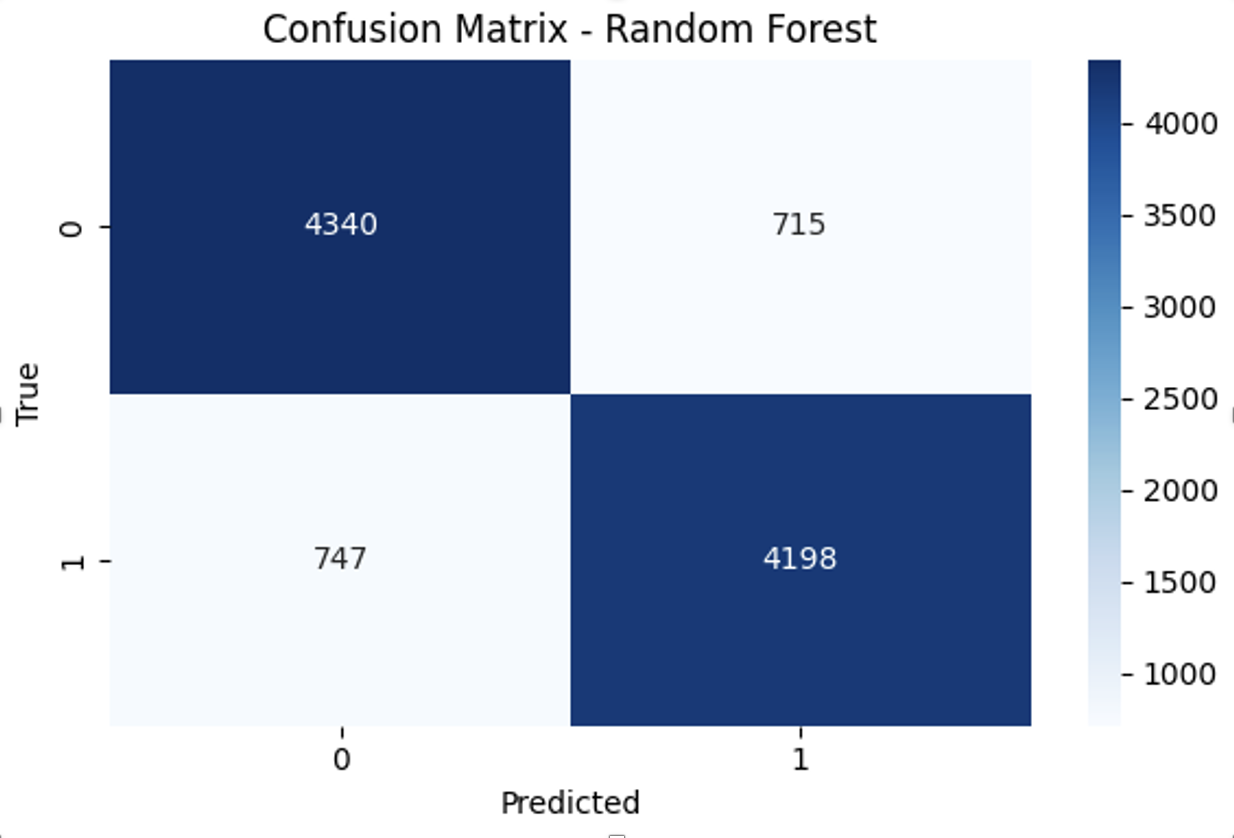
\includegraphics[width=0.4\textwidth]{pics/rf_eval_metrix.png}
    \caption{Confusion Matrix of Random Forest}
\end{figure}

Interpretation:
True Negatives (TN): 4340 — negative prediction correctly. \\
False Positives (FP): 715 — positive prediction incorrectly. \\
False Negatives (FN): 747 — negative prediction incorrectly. \\
True Positives (TP): 4198 — positive prediction correctly.

\subsection{Conclusion}
Random Forest proves to be a reliable and interpretable model for sentiment analysis of movie reviews. While deep learning methods may offer marginal gains, ensemble methods like Random Forest offer a good balance between performance and computational efficiency.


